% vim: et sw=2 ts=2 sts=2

\section{Heurísticas para Solução do Problema}
\frame{
  \frametitle{Heurísticas para Solução do Problema}
  \begin{block}{}
    \begin{enumerate}
      \item Lógica Nebulosa
      \item \textit{Conditional Random Fields} (CRFs)
      \item \textit{Ant Colony Optimization} (ACO)
      \item \textit{Simulated Annealing} (SA)
      \item Algorítimo Genético (AG)
      \item Redes Neurais
    \end{enumerate}
  \end{block}
}

\section{Logica Nebulosa}

\subsection{Introdução}

Sistemas nebulosos aproximam funções. Eles são aproximadores universais se usarem regras suficientes. 
Neste sentido sistemas difusos podem modelar qualquer função ou sistema contínuos. Aqueles sistemas 
podem vir tanto da física quanto da sociologia, bem como da teoria do controle ou do 
processamento de sinais.

A qualidade da aproximação difusa depende da qualidade das regras. Na prática especialistas sugerem regras
difusas ou aprendem-nas através de esquemas neurais através de dados e ajustam as regras com novos dados.
Os resultados sempre aproximam alguma função não linear desconhecida que pode mudar com o tempo. Melhores 
cérebros e melhores redes neurais resultam em melhores aproximações \cite{kosko1997fuzzy}.

\subsection{Modelo Aditivo Padrão(SAM)}

O sistema difuso $F:\Re^n \rightarrow \Re^p$ é em si uma árvore de regras rasa e extensa. É um aproximador
por antecipação. Existem $m$ regras da forma "Se $X$ é conjunto difuso $A$ então $Y$ é conjunto difuso $B$".
A partir desse nível o sistema depende cada vez menos em palavras. 

Cada entrada $x$ aciona parcialmente todas as regras em paralelo. Então o sistema age como um processador 
associativo a medida que calcula a saída
$F(x)$. 
%Definir a_j(x) e b_j(y)

Essas regras relacionam os conjuntos $A_j$ e $B_j$, gerando o caminho difuso $A_j x B_j$. Na prática,
é utilizado o produto para definir $ a_j x b_j (x,y) = a_j(x).b_j(y)$. Esta é a parte "padrão" no SAM.
A parte "aditiva" se refere ao fato de a entrada $x$ acionar a $j$-ésima regra em um grau $a_j(x)$ e o sistema 
soma os acionamentos ou partes escaladas dos conjuntos escalados $a_j(x)B_j$, conforme \cite{kosko1997fuzzy}:

\begin{eqnarray}
F(x) = \frac{\sum w_i.a_i(x).V_i.c_i}{\sum w_j.a_j(x).V_j}
\end{eqnarray}

Com o volume/área $V_j$ e o centroide $c_j$ são dados por:

\begin{eqnarray}
V_j = \int{b_j(y_1,...,y_p)}_{\Re^{p}}.dy_1...dy_p > 0\\
c_j = \frac{\int{y.b_j(y_1,...,y_p)}_{\Re^{p}}.dy_1...dy_p}{V_j}
\end{eqnarray}

\section{Conditional Random Fields}

\textit{Conditional Random Fields}, ou CRFs, são modelos de grafos não direcionados
utilizados para classificação estruturada. Os vértices são compostos por
observações, $X$, ou classes, $Y$.

A representação um dos aspectos fundamentais no problema de classificação de
dados sequenciais. Claramente, um modelo que suporta inferência tratável é
necessário, mas um modelo que representa os dados sem fazer suposições de
dependências não garantidas também é desejável. Um jeito de satisfazer ambos
os critérios é usar um modelo que define uma probabilidade condicional
$p(Y|x)$

Um caso particular dos CRF é quando as classes formam uma cadeia linear.
Isso pressupõem que a classificação atual só depende imediatamente da
anterior.

%
% Tradução do artigo: "Conditional Random Fields: An Introduction"
%

\subsection{Rotulamento de dados sequenciais}

A tarefa de rotular sequências para um conjunto de sequências de observações
surge em vários campos, incluindo bioinformática, linguística computacional
e reconhecimento de fala.

Um dos métodos mais comuns para executar tal tarefa de rotulamento e segmentação
é o emprego de \textit{Hidden Markov Models} (HMMs) ou autómato de estado finito
probabilístico para identificar a sequência de rótulos mais provável para qualquer
sequência de palavras dada. HMMs são uma forma de modelos generativa, que define
a distribuição de probabilidade conjunta $p(X,Y)$, onde $X$ e $Y$ são variáveis
aleatórias variando ao longo das sequências de observações e as correspondentes
sequências de rótulos. Com o objetivo de definir uma probabilidade conjunta dessa
natureza, os modelos generativos precisam enumerar todas as possíveis sequências de
observações - uma tarefa que, para alguns domínios, é intratável ao menos que os
elementos da observação forem representados por unidades isoladas, independente dos
outros elementos em uma sequencia de observações. Mais precisamente, um elemento
de observação em um dado instante no tempo só pode depender diretamente do estado,
ou rótulo, naquele tempo. Essa é uma suposição apropriada para poucos conjuntos de
dados simples, entretanto a maioria das sequencias de observação do mundo real são
bem representadas em termos de \textit{features} interativos múltiplos e dependências
de longo prazo elementos de observação.

Essa questão de representação é um dos problemas mais fundamentais do rotulamento de
dados sequenciais. Claramente, um modelo que suporte \textit{tractable inference} é
necessário, entretanto um moledo que represente os dados sem fazer suposições não
garantidas de independências também é desejável. Uma maneira de satisfazer ambos os
critérios é usar um modelo que define a probabilidade condicional $p(Y|x)$ ao longo
das sequências rotuladas dada uma sequência de observações particular $x$, ao invés de
um a distribuição conjunta ao longo de ambos as sequencias de rótulos e observações.
Modelos condicionais são usados para rotular uma sequência nova de observações $x_*$
selecionando uma sequência de rótulos $y_*$ que maximize a probabilidade condicional
$p(y_*|x_*)$. A natureza condicional de tais modelos significa que nenhum esforço é
perdido na modelagem das observações, e não é necessário fazer suposições não
garantidas de independência sobre o modelo. Atributos arbitrários dos dados observados
podem ser capturados, sem a necessidade do modelador ter que se preocupar como tais
atributos estão relacionados.

Campos aleatórios condicionais (CRFs) são \textit{frameworks} probabilísticas para
rotular e segmentar dados sequencias, baseado na abordagem condicional descrita no
parágrafo anterior. Um CRF é uma forma de modelo de grafo não direcionado que define
uma única distribuição \textit{log-linear} sobre sequências de rótulos dada uma
sequência de observações. A vantagem primária dos CRFs sobre os HMMs é a natureza
condicional, resultando em um \textbf{relachamento} das suposições de independência
necessárias pelos HMMs para garantir \textit{tractable inference}. Adicionalmente,
CRFs evitam o \textit{bias} de rotulamento, um problema dos modelos de máxima entropia
de Markov (MEMMs) e outros modelos de Markov condicionais baseados em modelos de grafos
direcionados. CRFs supera ambos os MEMMs e HMMs no número de tarefas de rotulamento de
sequências.

\subsection{Modelos Gráficos Não Direcionados}

Um CRF pode ser visto como um modelo gráfico não direcionado, ou um campo aleatório
de Markov, condicionado globalmente em \textbf{X}, a variável aleatória representando
as sequências de observações. Formalmente, define-se $G=(V,E)$ como sendo um
grafo não direcionado tal que exista um nó $v \in V$ correspondente a cada uma das
variáveis aleatórias representando um elemento $Y_v \in Y$. Se cada uma das variáveis
aleatórias $Y_v$ obedece a propriedade de Markov com relação a $G$, então $(Y,X)$ é
um CRF\@. Na teoria a estrutura do grafo $G$ pode ser arbitrária, desde que ele represente
as independências condicionais da sequência de rótulos sendo modelada. Entretanto,
ao se modelar as sequências, o grafo mais comum e simples encontrado é aquele cujos nós
correspondentes aos elementos de $Y$ formam uma cadeia linear de primeira ordem, conforme
ilustrado na figura~\ref{grafo_crf}.

<<incluir imagem>>

caption: Estrutura gráfica de CRFs de com estruturas em cadeia para sequências.
As variáveis correspondentes aos nós em braco não são geradas pelo modelo.

\subsection{Funções Potencias}

A estrutura gráfica de um CRF pode ser utilizada para fatorar a distribuição conjunta
ao longo dos elementos $Y_v$ de $Y$ em um produto normalizado de funções potencias de
valor real derivadas da noção de independência condicional. Cada função potencial
opera em um subconjunto das variáveis aleatórias representadas pelo vértices em $G$.
De acordo com a definição de independência condicional para um modelos gráficos não
direcionados, a ausência de uma aresta entre dois vértices em $G$ implica que as variáveis
aleatórias representadas por esses vértices são condicionalmente independentes dado todos
as outras variáveis aleatórias no modelo. A função potencial precisa garantir que é
possível fatorar a probabilidade conjunta de tal maneira que variáveis aleatórias
independentes não apareçam na mesma função potencial. A maneira mais fácil de satisfazer
esse requisito é impor à cada função potencial operar em um conjunto de variáveis aleatórias
cujos vértices correspondentes formam uma clique maximal em $G$. Isso garante que nenhuma
função potencial refira a qualquer par de variáveis aleatórias cujos vértices não são
diretamente conectados e, se dois vértices aparecem juntos em um clique essa relação é
explicitada. No caso de um CRF de com estruturas em cadeia, igual ao representado na
figura~\ref{grafo_crf}, cada função potencial irá operar em pares de variáveis rótulo adjacentes
$Y_i$ e $Y_{i+1}$.

É interessante notar que uma função potencial isolada não tem uma interpretação probabilística
isolada, entretanto representa restrições nas configurações das variáveis aleatórias nas quais
a função esta definida. Isso afeta a probabilidade de configurações globais - uma configuração
global com uma probabilidade maior tem mais chance de satisfazer mais restrições que uma
configuração global com baixa probabilidade.

\subsection{Modelagem Matemática}

Lafferty \textit{et al.} \cite{Lafferty} define a probabilidade de uma sequência particular
de rótulos $y$ dado a sequência de observações $x$ como sendo o produto de funções potenciais,
cada uma da forma:

\begin{eqnarray}
  exp(\sum_j \lambda_j t_j(y_{i-1},y_i,x,i) + \sum_k \mu_k s_k(y_i,x,i)),\label{crf_eq}
\end{eqnarray}

onde $t_j(y_{i-1},y_i,x,i)$ é uma \textit{feature transition function} do label em posições
$i$ e $i-1$ na sequência de rótulos; $s_k(y_i,x,i)$ é uma \textit{state feature function} do
rótulo na posição $i$ e da sequência de observação; e $\lambda_j$ e $\mu_k$ são parâmetros a
serem estimados dos dados de treinamento.

Quando se define as \textit{features function}, constrói-se um conjunto de funções com
contradomínio $R$ da forma $b(x,i)$ que extraem as \textit{features} das observações para
expressar alguma característica da distribuição empírica dos dados de treinamento que deveria
valer também para a distribuição do modelo. Um exemplo de tal \textit{feature} é:

\begin{eqnarray}
  b(x,i)=
  \left\{
    \begin{array}{rc}
      1, & \mbox{se a bola esta mais perto do time adversário}\\
      0, & \mbox{caso contrário}.
    \end{array}
  \right.
\end{eqnarray}

Cada \textit{feature function} pega um valor de uma das funções $b(x,i)$ se o estado atual
(no caso da função de estado) ou estado anterior e atual (no caso da função de transição)
assumam valores particulares. Todos as \textit{feature functions} são portanto de contradomínio
real. Por exemplo, considere as seguintes funções de transição:

\begin{eqnarray}
  t_j(y_{i-1},y_i,x,i)=
  \left\{
    \begin{array}{rc}
      b(x,i), & \mbox{se $y_{i-1}=IN$ e $y_i=NP$}\\
      0,      & \mbox{caso contrário}.
    \end{array}
  \right.
\end{eqnarray}

A seguinte notação simplificada será utilizada:

\begin{eqnarray}
  s(y_i,x,i)=s(y_{i-1},y_i,x,i)
\end{eqnarray}
e
\begin{eqnarray}
  F_j(y,x) = \sum_{i=1}^n f_j(y_{i-1},y_i,x,i),
\end{eqnarray}

Onde cada $f_j(y_{i-1},y_i,x,i)$ e ou uma função de estado $s(y_{i-1},y_i,x,i)$
ou uma função de transição $t(y_{i-1},y_i,x,i)$. Isso permite que a probabilidade
do rotulamento de uma sequência $y$ dado uma sequência de observações $x$ ser escrita
como:

\begin{eqnarray}
  p(y|x,\lambda) = \frac{1}{Z(x)} exp(\sum_j \lambda_j F_j(y,x)),
\end{eqnarray}

Onde $Z(x)$ é um fator de normalização.

\subsection{Máxima Entropia}

A forma de um CRF,mostrada em~\ref{crf_eq}, é fortemente motivada pelo princípio da
máxima entropia - um \textit{framework} para estimar distribuições de probabilidade
de um conjunto de dados de treinamento. A entropia de um conjunto de probabilidades
é uma medida de incerteza e é utilizada quando a distribuição em questão é a mais
uniforme possível. O princípio da máxima entropia afirma que a única distribuição
de probabilidade que pode justificavelmente ser construída de informação incompleta,
tal como um conjunto de dados finitos, é aquela que tem entropia máxima sujeita a
um conjunto de restrições que representam a informação disponível. Qualquer outra
distribuição vai envolver suposições não garantidas.

\subsection{Parâmetro de Inferência}

Assumindo que os dados de treinamento $\lbrace (x^{(k)},y^{(k)}) \rbrace$
são independentemente e identicamente distribuídos, o produto de~\ref{crf_eq}
sobre todas as sequências de treinamento, como uma função de parâmetro $\lambda$,
é conhecido como \textit{likelihood}, denotado por $p(\lbrace y^{(k)}\rbrace,\lbrace
x^{(k)}\rbrace, \lambda)$. Treinamentos que maximizam o \textit{likelihood} escolhem
valores de parâmetros tais que o logaritmo do \textit{likelihood}, também chamada de
\textit{log-likelihood}, seja máximo. Para um CRF, o \textit{log-likelihood} é dada por:

\begin{eqnarray}
  \mathcal{L}(\lambda) = \sum_k \left[ log\frac{1}{Z(x^{(k)})}+
    \sum_j \lambda_j F_j(y^{(k)},x^{(k)}) \right]
\end{eqnarray}

Não é possível determinar analiticamente a os valores dos parâmetros que maximizam
o \textit{log-likelihood}. Logo, para resolver essa equação dois métodos foram estudados
neste trabalho: \textit{ant colony optimization} e \textit{simulated annealing}.
Esse métodos são descritos nas próximas seções.

\frame{
  \frametitle{Otimização da Colonia de Formigas}
  \begin{block}{}
    \begin{figure}
      \centering
      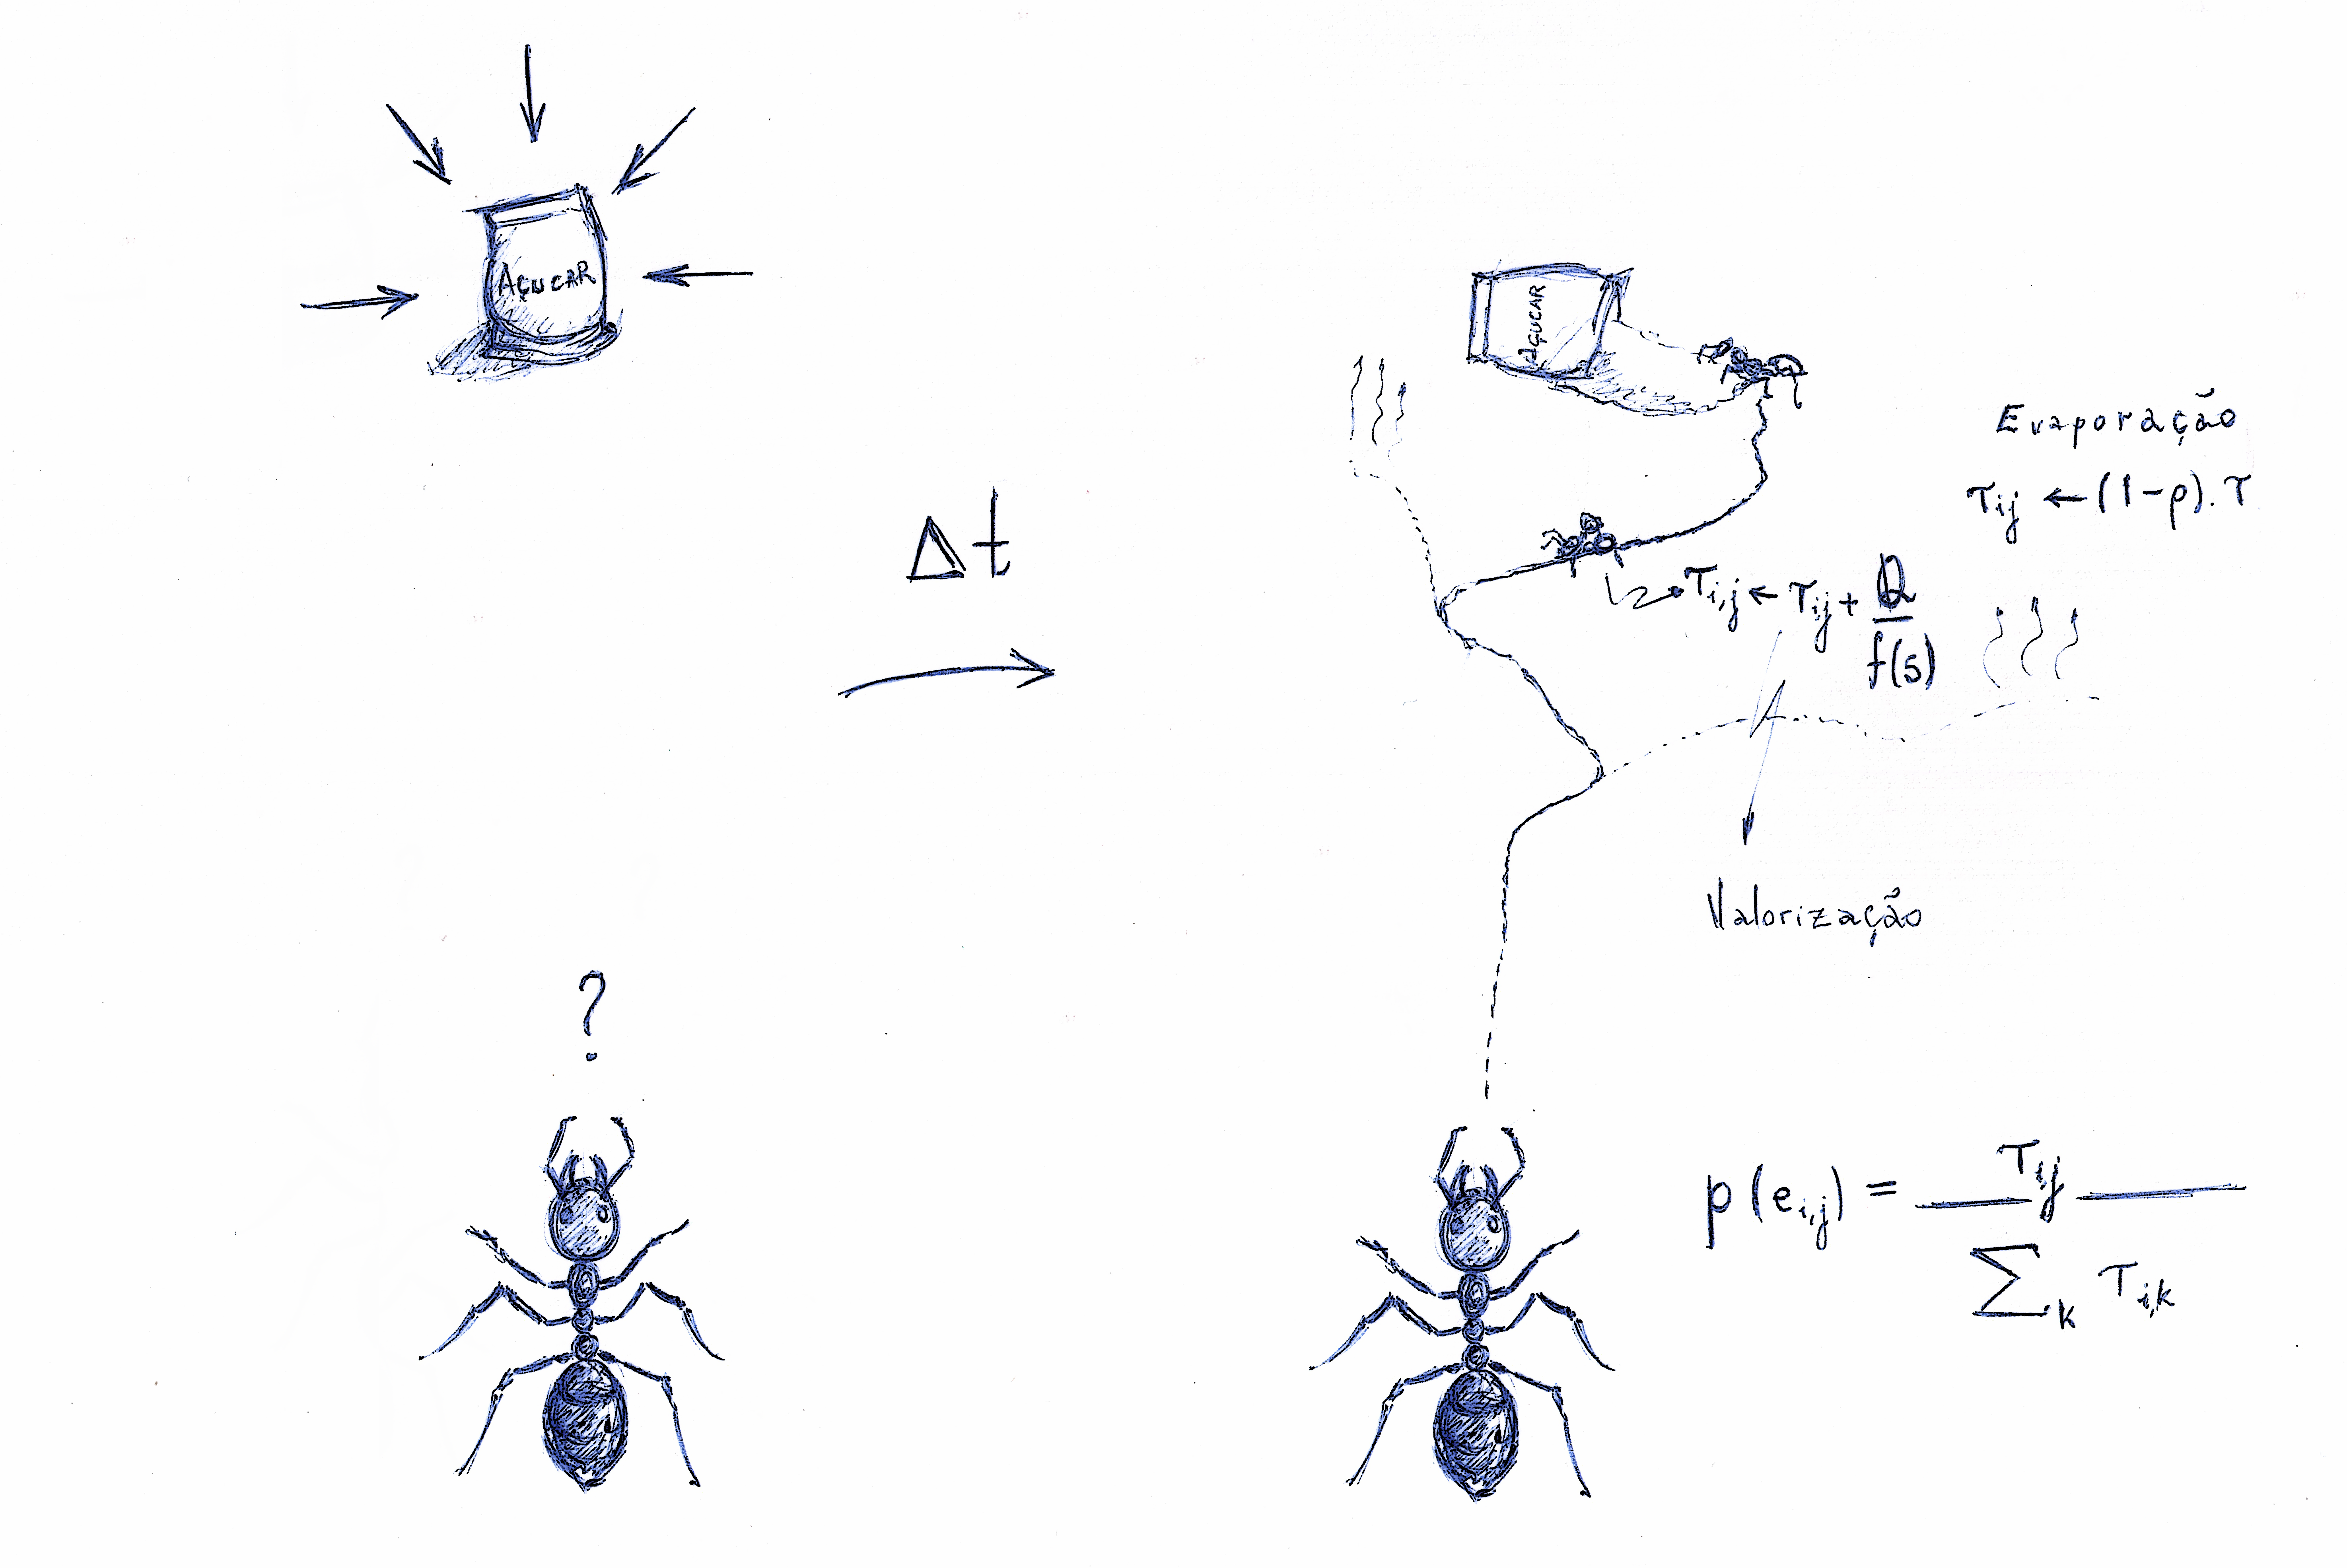
\includegraphics[width=0.8 \linewidth]
      {imgs/ilustrativa_aco}
      \caption{Idéia Básica do ACO}
    \end{figure}
  \end{block}
}

\frame{
  \frametitle{Otimização da Colonia de Formigas}
  \begin{block}{}
    \begin{figure}
      \centering
      \includegraphics[width=0.8 \linewidth]
      {imgs/meta_heuristica_aco}
      \caption{Diagrama de Funcionamento da Meta-Heurística do ACO}
    \end{figure}
  \end{block}
}

\frame{
  \frametitle{Otimização da Colonia de Formigas}
  \begin{block}{}
    \begin{figure}[ht]
      \includegraphics[width=0.4 \linewidth, height = 0.4 \linewidth]{imgs/exemplo_aco_1}
      \includegraphics[width=0.3 \linewidth, height = 0.4 \linewidth]{imgs/exemplo_aco_2}
      \includegraphics[width=0.3 \linewidth, height = 0.4 \linewidth]{imgs/exemplo_aco_3}

     \caption{Exemplo da construção da solução para o TSP problem}
    \end{figure}
  \end{block}
}
\frame{
  \frametitle{Recozimento Simulado}
  \begin{block}{}
    \begin{figure}
      \centering
      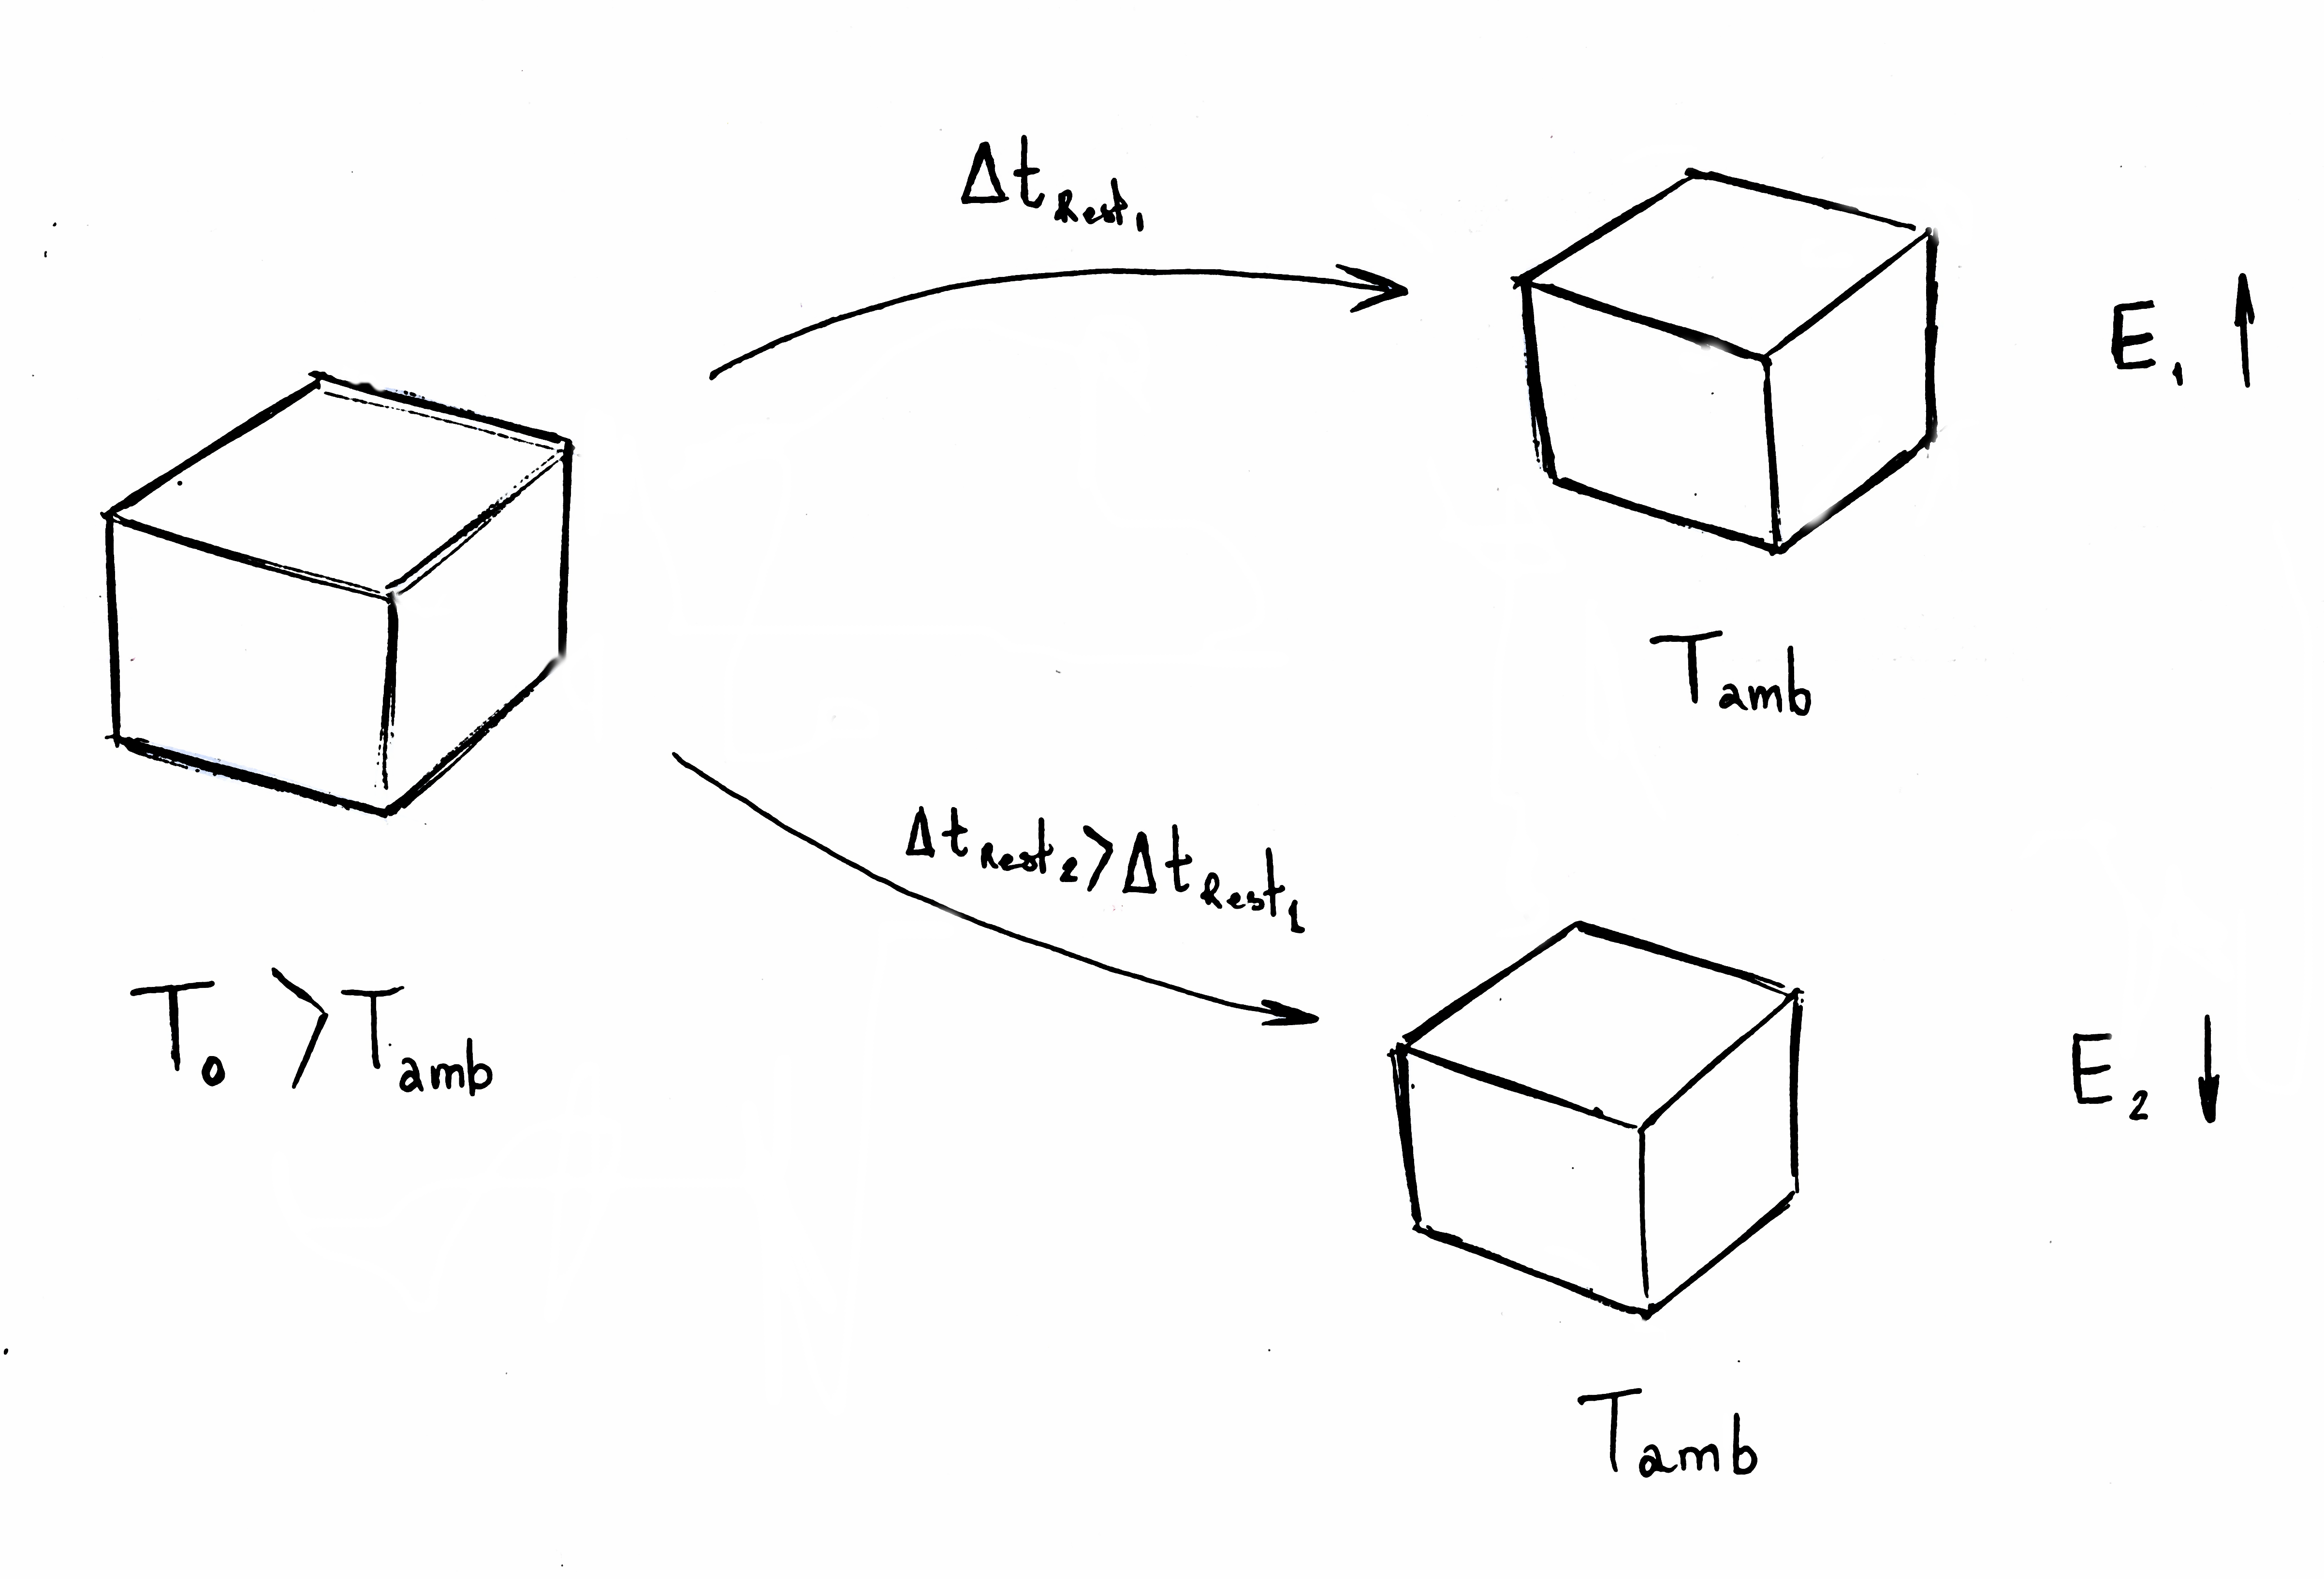
\includegraphics[width = 0.6 \linewidth]{imgs/ilustrativa_sa}
      \caption{Idéia Básica do SA}
    \end{figure}
  \end{block}
}

\frame{
  \frametitle{Recozimento Simulado}
  \begin{block}{}
    \begin{figure}
      \centering
      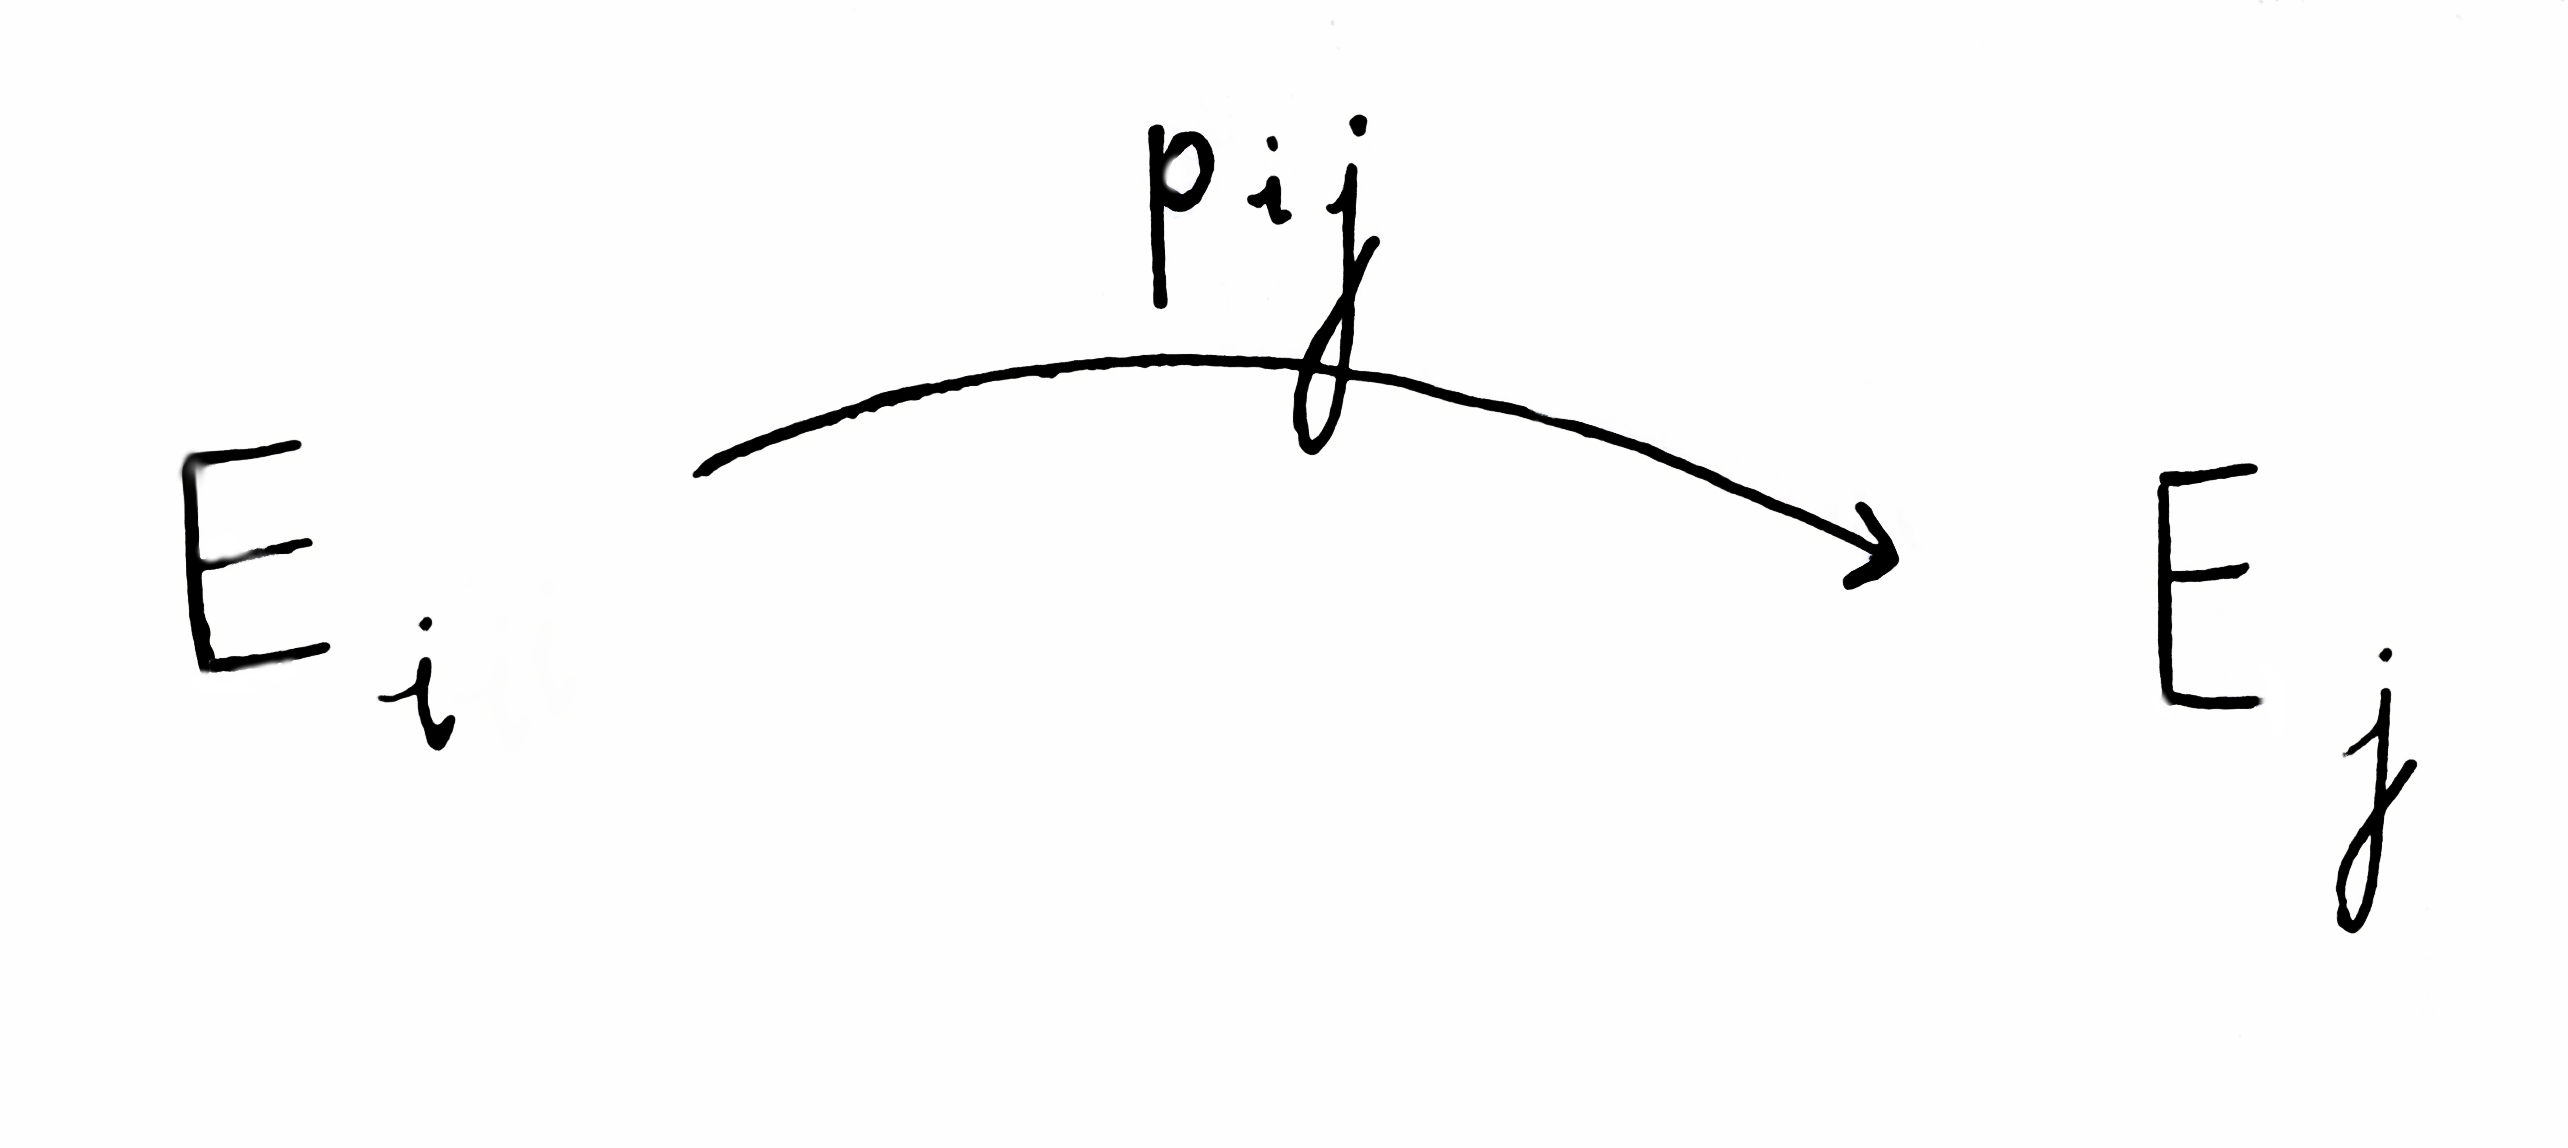
\includegraphics[width = 0.5 \linewidth]{imgs/transicao_sa}
      \caption{Probabilidade da Transição do Estado $i$ para o Estado $j$}
    \end{figure}
  \end{block}
  \begin{block}{}
    $$p_{ij}=\left\{\begin{array}{rc}
    1,&\mbox{se}\quad E\lbrace r_j \rbrace \le E\lbrace r_i \rbrace\\
    e^{\frac{- E\lbrace r_j \rbrace - E\lbrace r_i \rbrace}{k_B T} }, &\mbox{se}\quad 
    E\lbrace r_j \rbrace > E\lbrace r_i \rbrace
    \end{array}\right.
    $$
  \end{block}
}

\frame{
  \frametitle{Recozimento Simulado}
  \begin{block}{}
    Elementos básicos do SA:
    \begin{itemize}
      \item $S$, espaço de estado finito
      \item $J: S \rightarrow \mathbb{R}$, função de custo
      \item $S(i) \subset S - \lbrace i \rbrace$ para cada $i \in S$
      \item $q_{ij}, j \in S(i)$, tal que $\sum_{j \in S_{i}} q_{ij} = 1$
      \item $T: \mathbb{N} \rightarrow (0, \infty)$, rotina de resfriamento
      \item $x(0) \in S$, estado inicial
    \end{itemize}
  \end{block}
}
\frame{
\frametitle{Algoritmo Genético}
\begin{block}{}

%\begin{lstlisting}
\begin{algorithm}[H]
\SetKwBlock{Procedimento}{Procedimento}{fim}

%Algorithm: GA(n, \ki, \mu)
\Procedimento{
  %// Initialise generation 0:
  $k \leftarrow 0$, $P_k \leftarrow n$ indivíduos aleatórios\;
  %// EvaluatePk:
  %\Para{cada $i$ em $P_k$}
  %Compute fitness(i) for each i ∈ Pk;
  %Computar a $avaliacao(i)$ para cada $i$ em $P_k$\;
  %while fitness of fittest individual in Pk is not high enough;
  %\Enqto{a $avaliacao(i)$ de cada $i$ em $P_k$ não for boa o suficiente}{
  \Enqto{$avaliacao(i) < desejado$ de cada $i$ em $P_k$}{
    %// Create generation k + 1:
    %// 1. Copy:
    %Select (1−χ)×n members ofPk and insert into Pk+1;
    Selecionar os $(1 - \chi) \times n$ membros com maior $avaliacao(i)$ de $P_k$ e inserir em $P_{k+1}$\;
    %// 2. Crossover:
    %Select χ×n members of Pk; pair them up; produce offspring; insert the offspring into Pk+1;
    Selecionar $\chi \times n$ membros de $P_k$, pareá-los e inserir a cria em $P_{k+1}$\;
    %// 3. Mutate:
    %Select µ×n members of Pk+1; invert a randomly-selected bit in each;
    Selecionar os $\mu \times n$ membros de $P_{k+1}$ com maior $avaliacao(i)$ e inverter um bit aleatório de cada membro\;
    %// Evaluate Pk+1:
    %Compute fitness(i) for each i ∈ Pk;
    %Computar a $avaliacao(i)$ para cada $i$ em $P_{k+1}$\;
    %// Increment:
    %k := k + 1;
    $k \leftarrow k + 1$\;
  }
%return the fittest individual from Pk;ut your code here.
  \Retorna{membro $i$ em $P_k$ com maior $avaliacao(i)$}
}
\caption{Pseudo código de um Algoritmo Genético}
\end{algorithm}
\end{block}
}

\frame{
\frametitle{Redes Neurais}
\begin{block}{}
\begin{figure}[H]
\centering
\includegraphics[width=10cm]{figuras/rede_neural_neuronio}
\caption{Modelo matemático de um neurônio.}
\end{figure}
\end{block}
}

\frame{
\frametitle{Redes Neurais}
\begin{block}{}
\begin{figure}[H]
\centering
\includegraphics[width=10cm]{figuras/rede_neural_simple_problem}
\caption{\textit{Perceptron} para decidir região de um ponto no plano.}
\end{figure}
\end{block}
}

\frame{
\frametitle{Redes Neurais}
\begin{block}{}
\begin{figure}[H]
\centering
\includegraphics[width=10cm]{figuras/rede_neural_linear_probl}
\caption{Problemas linearmente separáveis vs. não linearmente separáveis.}
\end{figure}
\end{block}
}

\frame{
\frametitle{Redes Neurais}
\begin{block}{}
\begin{figure}[H]
\centering
\includegraphics[width=8cm]{figuras/rede_neural_topologia}
\caption{Topoligia de camadas.}
\end{figure}
\end{block}
}
